% Options for packages loaded elsewhere
\PassOptionsToPackage{unicode}{hyperref}
\PassOptionsToPackage{hyphens}{url}
\PassOptionsToPackage{dvipsnames,svgnames,x11names}{xcolor}
%
\documentclass[
  letterpaper,
  DIV=11,
  numbers=noendperiod]{scrartcl}

\usepackage{amsmath,amssymb}
\usepackage{iftex}
\ifPDFTeX
  \usepackage[T1]{fontenc}
  \usepackage[utf8]{inputenc}
  \usepackage{textcomp} % provide euro and other symbols
\else % if luatex or xetex
  \usepackage{unicode-math}
  \defaultfontfeatures{Scale=MatchLowercase}
  \defaultfontfeatures[\rmfamily]{Ligatures=TeX,Scale=1}
\fi
\usepackage{lmodern}
\ifPDFTeX\else  
    % xetex/luatex font selection
\fi
% Use upquote if available, for straight quotes in verbatim environments
\IfFileExists{upquote.sty}{\usepackage{upquote}}{}
\IfFileExists{microtype.sty}{% use microtype if available
  \usepackage[]{microtype}
  \UseMicrotypeSet[protrusion]{basicmath} % disable protrusion for tt fonts
}{}
\makeatletter
\@ifundefined{KOMAClassName}{% if non-KOMA class
  \IfFileExists{parskip.sty}{%
    \usepackage{parskip}
  }{% else
    \setlength{\parindent}{0pt}
    \setlength{\parskip}{6pt plus 2pt minus 1pt}}
}{% if KOMA class
  \KOMAoptions{parskip=half}}
\makeatother
\usepackage{xcolor}
\setlength{\emergencystretch}{3em} % prevent overfull lines
\setcounter{secnumdepth}{-\maxdimen} % remove section numbering
% Make \paragraph and \subparagraph free-standing
\makeatletter
\ifx\paragraph\undefined\else
  \let\oldparagraph\paragraph
  \renewcommand{\paragraph}{
    \@ifstar
      \xxxParagraphStar
      \xxxParagraphNoStar
  }
  \newcommand{\xxxParagraphStar}[1]{\oldparagraph*{#1}\mbox{}}
  \newcommand{\xxxParagraphNoStar}[1]{\oldparagraph{#1}\mbox{}}
\fi
\ifx\subparagraph\undefined\else
  \let\oldsubparagraph\subparagraph
  \renewcommand{\subparagraph}{
    \@ifstar
      \xxxSubParagraphStar
      \xxxSubParagraphNoStar
  }
  \newcommand{\xxxSubParagraphStar}[1]{\oldsubparagraph*{#1}\mbox{}}
  \newcommand{\xxxSubParagraphNoStar}[1]{\oldsubparagraph{#1}\mbox{}}
\fi
\makeatother


\providecommand{\tightlist}{%
  \setlength{\itemsep}{0pt}\setlength{\parskip}{0pt}}\usepackage{longtable,booktabs,array}
\usepackage{calc} % for calculating minipage widths
% Correct order of tables after \paragraph or \subparagraph
\usepackage{etoolbox}
\makeatletter
\patchcmd\longtable{\par}{\if@noskipsec\mbox{}\fi\par}{}{}
\makeatother
% Allow footnotes in longtable head/foot
\IfFileExists{footnotehyper.sty}{\usepackage{footnotehyper}}{\usepackage{footnote}}
\makesavenoteenv{longtable}
\usepackage{graphicx}
\makeatletter
\def\maxwidth{\ifdim\Gin@nat@width>\linewidth\linewidth\else\Gin@nat@width\fi}
\def\maxheight{\ifdim\Gin@nat@height>\textheight\textheight\else\Gin@nat@height\fi}
\makeatother
% Scale images if necessary, so that they will not overflow the page
% margins by default, and it is still possible to overwrite the defaults
% using explicit options in \includegraphics[width, height, ...]{}
\setkeys{Gin}{width=\maxwidth,height=\maxheight,keepaspectratio}
% Set default figure placement to htbp
\makeatletter
\def\fps@figure{htbp}
\makeatother

\usepackage{booktabs}
\usepackage{caption}
\usepackage{longtable}
\usepackage{colortbl}
\usepackage{array}
\usepackage{anyfontsize}
\usepackage{multirow}
\KOMAoption{captions}{tableheading}
\makeatletter
\@ifpackageloaded{caption}{}{\usepackage{caption}}
\AtBeginDocument{%
\ifdefined\contentsname
  \renewcommand*\contentsname{Table of contents}
\else
  \newcommand\contentsname{Table of contents}
\fi
\ifdefined\listfigurename
  \renewcommand*\listfigurename{List of Figures}
\else
  \newcommand\listfigurename{List of Figures}
\fi
\ifdefined\listtablename
  \renewcommand*\listtablename{List of Tables}
\else
  \newcommand\listtablename{List of Tables}
\fi
\ifdefined\figurename
  \renewcommand*\figurename{Figure}
\else
  \newcommand\figurename{Figure}
\fi
\ifdefined\tablename
  \renewcommand*\tablename{Table}
\else
  \newcommand\tablename{Table}
\fi
}
\@ifpackageloaded{float}{}{\usepackage{float}}
\floatstyle{ruled}
\@ifundefined{c@chapter}{\newfloat{codelisting}{h}{lop}}{\newfloat{codelisting}{h}{lop}[chapter]}
\floatname{codelisting}{Listing}
\newcommand*\listoflistings{\listof{codelisting}{List of Listings}}
\makeatother
\makeatletter
\makeatother
\makeatletter
\@ifpackageloaded{caption}{}{\usepackage{caption}}
\@ifpackageloaded{subcaption}{}{\usepackage{subcaption}}
\makeatother

\ifLuaTeX
  \usepackage{selnolig}  % disable illegal ligatures
\fi
\usepackage{bookmark}

\IfFileExists{xurl.sty}{\usepackage{xurl}}{} % add URL line breaks if available
\urlstyle{same} % disable monospaced font for URLs
\hypersetup{
  pdftitle={EDRM 718 Adam Brown Final Project},
  pdfauthor={Adam Brown},
  colorlinks=true,
  linkcolor={blue},
  filecolor={Maroon},
  citecolor={Blue},
  urlcolor={Blue},
  pdfcreator={LaTeX via pandoc}}


\title{EDRM 718 Adam Brown Final Project}
\author{Adam Brown}
\date{2025-05-01}

\begin{document}
\maketitle


\subsection{Description}\label{description}

This research report explores the relationships between optimism scores
(from the survey data and measures their outlook on employment and
career readiness), reported GPAs, and the college students academic
disciplines or subjects. More specifically, this report seeks to answer
these three questions, Is senior-year grade point average (GPA) related
to the degree of optimism about future employment? Is the relationship
of GPA and optimism consistent or different for different categories of
disciplines? Is the level of optimism different for different categories
of disciplines? The three datasets include survey results from over 700
college seniors. graduating this spring, representing 23 major
universities in the United States. These datasets include demographic
data, academic performance data, and data from a short (14-item)
Likert-type survey which sought to determine their optimism regarding
their readiness and likelihood of obtaining a job after graduation

\textbf{Source of Data:} Real World Solutions, Job Prep Demographics,
Job Prep GPA, and Job Prep Survey Results. Sourced 24 April 2025.

\subsection{Analysis}\label{analysis}

I begin my analysis reading in the three separate data files, tidying
the data that is missing or has problems, and then joining the files
together using my unique key, which in this case is Student ID number.
Now that I have completed the data processing and cleaning, I start by
examining the reported GPAs for the students from the first and second
semester. We need to verify consistency of GPAs before we can create a
weighted GPA average.

In Figure 1, I created a scatterplot to verify consistency by observing
if there a strong linear relationship exists between first and second
semester GPAs. In Figure 1, we observe that as the GPA for the first
semester increases, so does the GPA for the second semester. This tell
us that a strong linear relationship does exist. Since a strong linear
relationship exists this GPAs are comparable which means we can create
our next scatterplot which will helps us to know if we can predict
second semester GPA from first semester GPA.

\paragraph{Figure 1. Scatterplot of First Semester GPA Vs Second
Semester
GPA.}\label{figure-1.-scatterplot-of-first-semester-gpa-vs-second-semester-gpa.}

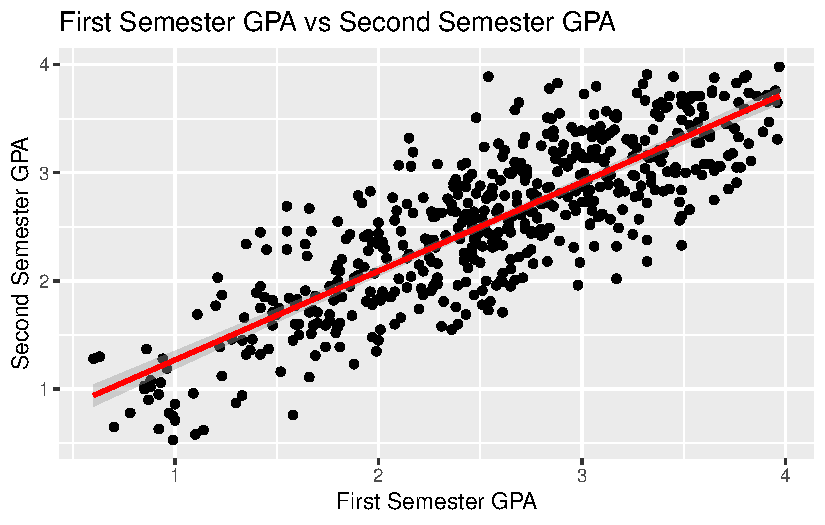
\includegraphics{EDRM-718-Adam-Brown-Final-Project_files/figure-pdf/unnamed-chunk-10-1.pdf}

In Figure 2, I created a scatterplot to identify if patterns exist or
not. We do not observe any shapes or patters in the data, which is good
because this means the residuals are randomly distributed. This
scatterplot helps me to know that my linear model is a good fit and
there shouldn't be significant bias in predicting second semester GPA
from first semester. This gives me confidence to create a weighted GPA
but first I need to identify and exclude those students who are among
those with the ten percent largest residuals. I run this analysis next
in Figure 3.

\paragraph{Figure 2. Scatterplot of Residuals from Predicted Second
Semester
GPA.}\label{figure-2.-scatterplot-of-residuals-from-predicted-second-semester-gpa.}

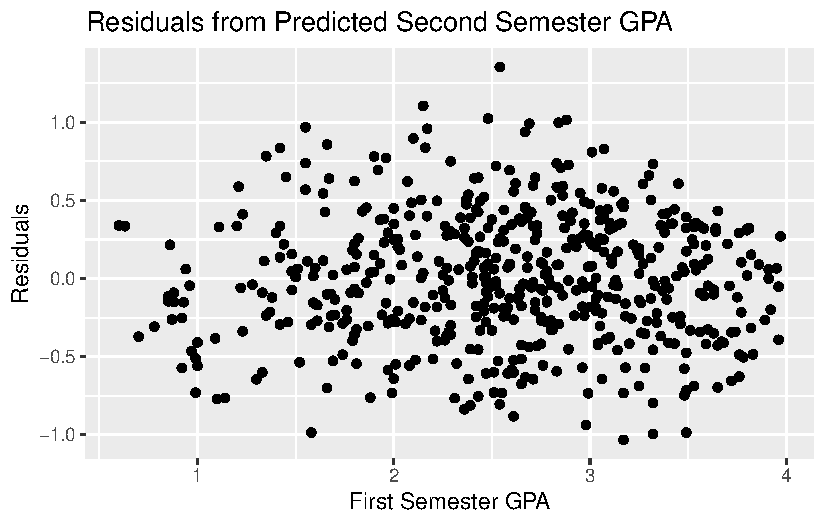
\includegraphics{EDRM-718-Adam-Brown-Final-Project_files/figure-pdf/unnamed-chunk-11-1.pdf}

In Figure 3, we can observe the students who are among those with the
ten percent largest residuals as they are noted in red. We note from our
data that there are 54 students who fall into this category. I will
remove those students from the data prior to calculating weighted GPA,
which we will call ``Senior Year GPA'' and we will continue to move
through the analysis.

\paragraph{Figure 3. Scatterplot of First Semester GPA Vs Second
Semester GPA with Large
Residuals.}\label{figure-3.-scatterplot-of-first-semester-gpa-vs-second-semester-gpa-with-large-residuals.}

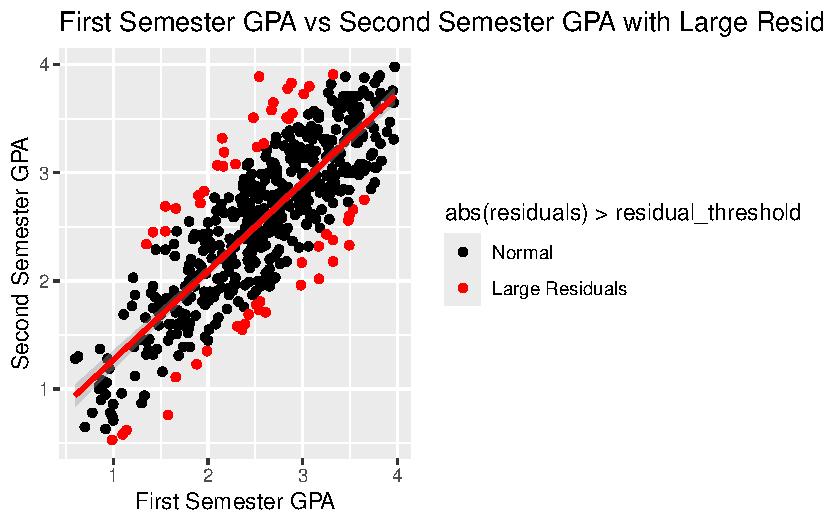
\includegraphics{EDRM-718-Adam-Brown-Final-Project_files/figure-pdf/unnamed-chunk-13-1.pdf}

\paragraph{Analysis for Question \#1: Is Senior-year Grade Point Average
(GPA) Related to the Degree of Optimism about Future
Employment?}\label{analysis-for-question-1-is-senior-year-grade-point-average-gpa-related-to-the-degree-of-optimism-about-future-employment}

In figure 4, we start to answer our first research question, Is
senior-year grade point average (GPA) related to the degree of optimism
about future employment? We start by verifying consistency by reviewing
the ten students with the largest residuals in the dataset. We can
observe these students by the red dots in Figure 4. We analyze these
residuals further in Figure 5.

\paragraph{Figure 4. Scatterplot of Residuals of Senior Year GPA Vs
Optimism
Score.}\label{figure-4.-scatterplot-of-residuals-of-senior-year-gpa-vs-optimism-score.}

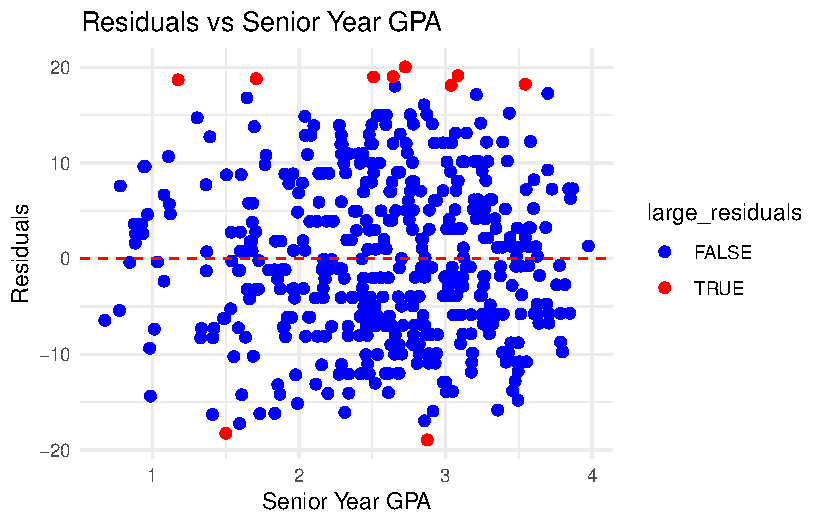
\includegraphics{EDRM-718-Adam-Brown-Final-Project_files/figure-pdf/unnamed-chunk-17-1.pdf}

In Figure 5, we further explore the residuals to ensure consistency
prior to running more analysis. Again, we observe a similar trend in the
data in the Histogram that we did in Figure 4. There are a few students
who have higher residuals, however, after reviewing these students in
the dataset, they show no discernible pattern between them on Subjects,
GPA, Optimism Score, etc. So, it will not strengthen our model to remove
these students, thus we retain them in the dataset.

\paragraph{Figure 5. Histogram of the Frequency of Absolute
Residuals.}\label{figure-5.-histogram-of-the-frequency-of-absolute-residuals.}

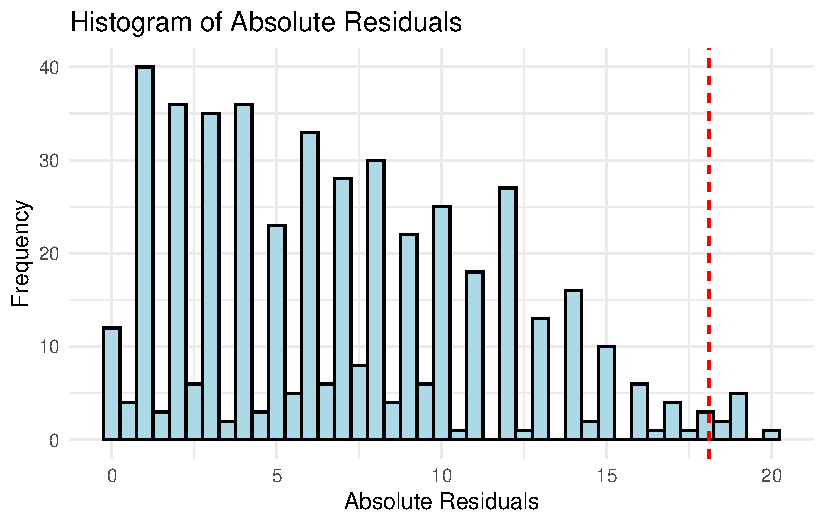
\includegraphics{EDRM-718-Adam-Brown-Final-Project_files/figure-pdf/unnamed-chunk-18-1.pdf}

In Figure 6, we observe the scatterplot of Senior Year GPA vs Optimism
Score. From our observations, it appears there is not a strong
relationship between the two variables. Meaning that as GPA increases,
optimism scores does not necessarily increase or decrease. We examine
these variables further in Table 1.

\paragraph{Figure 6. Scatterplot of Senior Year GPA (Weighted GPA) Vs
Optimism
Score.}\label{figure-6.-scatterplot-of-senior-year-gpa-weighted-gpa-vs-optimism-score.}

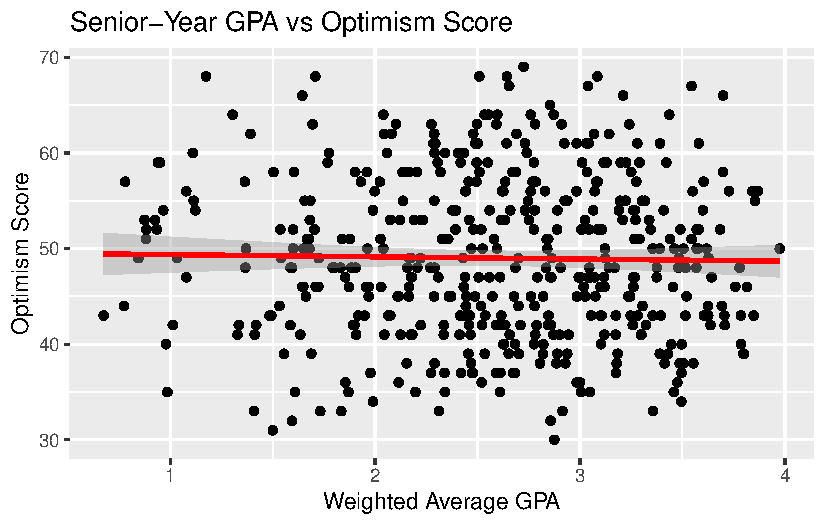
\includegraphics{EDRM-718-Adam-Brown-Final-Project_files/figure-pdf/unnamed-chunk-19-1.pdf}

In Table 1, we observe the correlation coefficient between Senior Year
GPA and Optimism score. , Based on the coefficient, there is a very
small and negative relationship between these two variables. As we
predicted from Figure 6, no strong relationship exists. To be sure, we
run one more analysis in Table 2.

\paragraph{Table 1. Correlation Between Senior Year GPA and Optimism
Score.}\label{table-1.-correlation-between-senior-year-gpa-and-optimism-score.}

\begin{table}
\caption*{
{\large Correlation Between Weighted GPA and Optimism Score}
} 
\fontsize{12.0pt}{14.4pt}\selectfont
\begin{tabular*}{\linewidth}{@{\extracolsep{\fill}}llr}
\toprule
Variable 1 & Variable 2 & Correlation\_Coefficient \\ 
\midrule\addlinespace[2.5pt]
weighted\_avg\_gpa & total\_score & -0.02 \\ 
\bottomrule
\end{tabular*}
\end{table}

In Table 2, we again learn that there is a small negative relationship
between the two variables and this helps us answer no to the question:
Is senior-year grade point average (GPA) related to the degree of
optimism about future employment?

\paragraph{Table 2. Linear Regression of Optimism Score and Senior Year
GPA.}\label{table-2.-linear-regression-of-optimism-score-and-senior-year-gpa.}

\begin{table}
\caption*{
{\large Linear Regression Results: Optimism Score vs Weighted GPA}
} 
\fontsize{12.0pt}{14.4pt}\selectfont
\begin{tabular*}{\linewidth}{@{\extracolsep{\fill}}lrrrr}
\toprule
Term & Estimate & Standard Error & t-Statistic & p-Value \\ 
\midrule\addlinespace[2.5pt]
(Intercept) & 49.60 & 1.45 & 34.12 & 0.00 \\ 
weighted\_avg\_gpa & -0.23 & 0.54 & -0.42 & 0.67 \\ 
\bottomrule
\end{tabular*}
\end{table}

\paragraph{Analysis for Question \#2: Is the Relationship of GPA and
Optimism Consistent or Different for Different Categories of
Disciplines?}\label{analysis-for-question-2-is-the-relationship-of-gpa-and-optimism-consistent-or-different-for-different-categories-of-disciplines}

In figure 6, we observe the relationship between Senior Year GPA and
Optimism Score is not consistent across different subjects or
disciplines. For example, we note that they relationship between Senior
Year GPA and Optimism Score in some subjects, like Humanities and
Natural Sciences, appears to be negative. However, subjects like Applied
Sciences and Social Sciences appear to have a weak or negative
relationship with Optimism Score. To be more conclusive, we examine this
question further in Table 3 with Linear Regression of Subjects.

\paragraph{Figure 6. Scatterplot of Senior Year GPA Vs Optimism Score by
Subject.}\label{figure-6.-scatterplot-of-senior-year-gpa-vs-optimism-score-by-subject.}

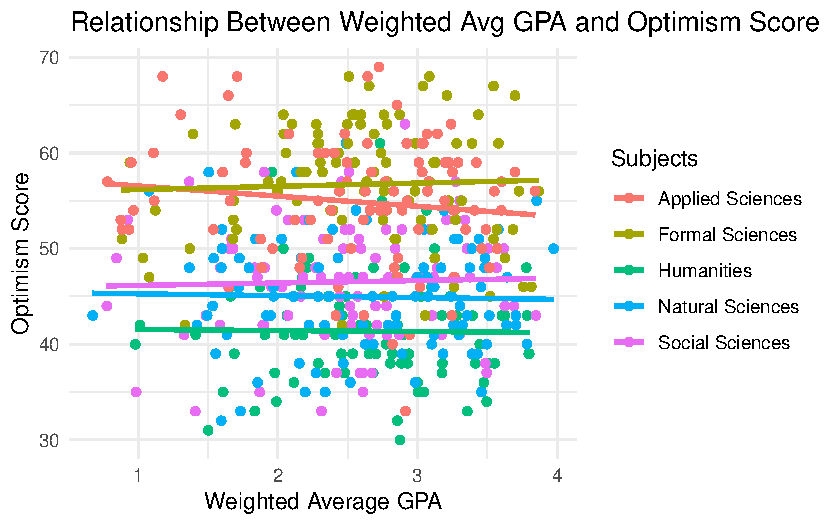
\includegraphics{EDRM-718-Adam-Brown-Final-Project_files/figure-pdf/unnamed-chunk-22-1.pdf}

In Table 3, we further seek to answer the question, Is the relationship
of GPA and optimism consistent or different for different categories of
disciplines? We learn from the linear regression in Table 3, with either
negative or small coefficients for each subject, that the relationship
must in fact be different for different categories of disciplines.
However, we run one more test to be sure in Table 4, an interaction
model between Optimism Score and Senior Year GPA by Subject.

\paragraph{Table 3. Linear Regression of
Subjects.}\label{table-3.-linear-regression-of-subjects.}

\begin{table}
\caption*{
{\large Linear Regression Model Results by Subject}
} 
\fontsize{12.0pt}{14.4pt}\selectfont
\begin{tabular*}{\linewidth}{@{\extracolsep{\fill}}lrr}
\toprule
Subject & Coefficient of Senior Year GPA & p-value \\ 
\midrule\addlinespace[2.5pt]
Applied Sciences & -1.06 & 0.24 \\ 
Formal Sciences & 0.34 & 0.70 \\ 
Humanities & -0.11 & 0.91 \\ 
Natural Sciences & -0.19 & 0.80 \\ 
Social Sciences & 0.25 & 0.77 \\ 
\bottomrule
\end{tabular*}
\end{table}

In table 4, we observe the interaction model (Relationship) of Optimism
Score and Senior Year GPA across different subjects. We observe, like in
Figure 6, the relationship is indeed different across different subjects
and mostly negative when comparing each subject to Applied Sciences for
Optimism Score. Meaning that in general as GPA increases and is held
constant, Optimism Scores decreases. However, based on the interaction
data with the subjects in Table 4, we learn that there is a positive
relationship for all subjects when compared to Applied Sciences. This
tells us that the interaction between Senior Year GPA and Optimism Score
is stronger in all subjects compared to Applied Sciences. The good news
that from Table 4 we can interpret the confidence intervals and
determine with 95\% confidence where we would expect a score to be. For
example, we can predict with 95\% confidence that when GPA is held
constant, an optimism score for Social Sciences will fall between -17.95
and -5.48. This confidence interval does not include zero, meaning it is
statistically significant. However, for the confidence intervals that do
include zero, these would not be considered statically significant. In
summary, Is the relationship of GPA and optimism consistent or different
for different categories of disciplines? Yes, it is different for
different categories of disciplines.

\paragraph{Table 4. Interaction Model of Optimism Score Vs Senior Year
GPA, and
Subjects.}\label{table-4.-interaction-model-of-optimism-score-vs-senior-year-gpa-and-subjects.}

\begin{table}
\caption*{
{\large Interaction Model Results: Optimism Score vs Senior Year GPA and Subjects}
} 
\fontsize{12.0pt}{14.4pt}\selectfont
\begin{tabular*}{\linewidth}{@{\extracolsep{\fill}}lrrrrrr}
\toprule
Term & Estimate & Standard Error & t-Statistic & p-Value & 95\% CI Lower & 95\% CI Upper \\ 
\midrule\addlinespace[2.5pt]
(Intercept) & 57.61 & 2.21 & 26.11 & 0.00 & 53.27 & 61.95 \\ 
weighted\_avg\_gpa & -1.06 & 0.83 & -1.28 & 0.20 & -2.69 & 0.56 \\ 
SubjectsFormal Sciences & -1.78 & 3.21 & -0.55 & 0.58 & -8.08 & 4.52 \\ 
SubjectsHumanities & -15.97 & 3.58 & -4.46 & 0.00 & -23.00 & -8.94 \\ 
SubjectsNatural Sciences & -12.15 & 3.13 & -3.89 & 0.00 & -18.29 & -6.00 \\ 
SubjectsSocial Sciences & -11.72 & 3.17 & -3.69 & 0.00 & -17.95 & -5.48 \\ 
weighted\_avg\_gpa:SubjectsFormal Sciences & 1.40 & 1.19 & 1.18 & 0.24 & -0.94 & 3.74 \\ 
weighted\_avg\_gpa:SubjectsHumanities & 0.96 & 1.32 & 0.72 & 0.47 & -1.65 & 3.56 \\ 
weighted\_avg\_gpa:SubjectsNatural Sciences & 0.87 & 1.16 & 0.75 & 0.46 & -1.42 & 3.16 \\ 
weighted\_avg\_gpa:SubjectsSocial Sciences & 1.32 & 1.21 & 1.08 & 0.28 & -1.07 & 3.70 \\ 
\bottomrule
\end{tabular*}
\end{table}

\paragraph{Analysis for Question \#3: Is the Level of Optimism Different
for Different Categories of
Disciplines?}\label{analysis-for-question-3-is-the-level-of-optimism-different-for-different-categories-of-disciplines}

In Figure 8 we can observe the following in relationship to our
question, Is the level of optimism different for different categories of
disciplines?, students in applied and formal sciences appear to have
higher and more consistent levels of optimism when compared with
students in humanities or natural sciences. In addition, students in the
social sciences discipline have higher variability than other
disciplines, meaning some student are very optimistic while others are
very pessimistic. I will run more analysis on this data in Table 5 by
running an ANOVA test.

\paragraph{Figure 8. Distribution of Optimism Scores Across
Subjects.}\label{figure-8.-distribution-of-optimism-scores-across-subjects.}

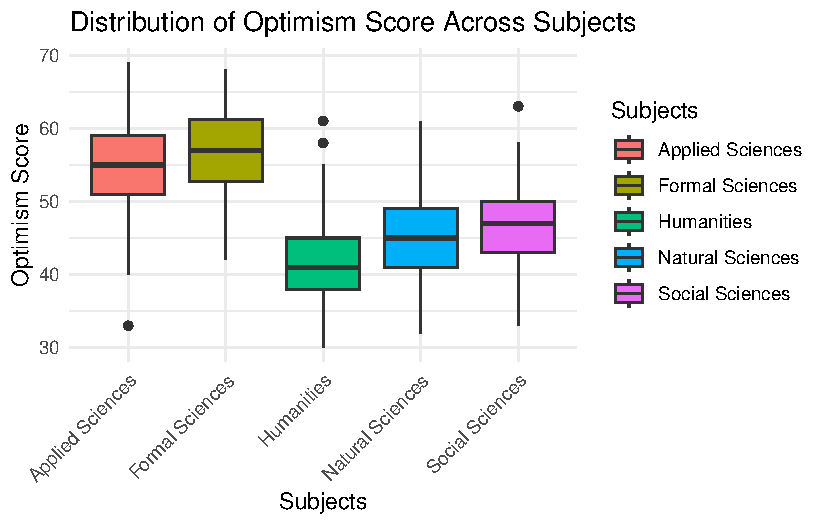
\includegraphics{EDRM-718-Adam-Brown-Final-Project_files/figure-pdf/unnamed-chunk-25-1.pdf}

In table 5, we observe a one-way ANOVA test of Optimism Scores across
different subjects to help us continue to answer our research question.
In this table we observe an F-value of 114.10 which is quite large and
tells us there is a strong relationship between Subjects and Optimism
Scores and that the level of optimism about future employment differs
significantly based on the subject. The observed P value also tell us
that this could be statistically significant, and we would normally
reject the null hypothesis of: there is no observed difference in
optimism scores across subjects. However, in the next table we run 95\%
confidence intervals which will tell us with greater confidence.

\paragraph{Table 5. One-way ANOVA of Optimism Score Across
Subjects.}\label{table-5.-one-way-anova-of-optimism-score-across-subjects.}

\begin{table}
\caption*{
{\large ANOVA Results for Optimism Score by Subject}
} 
\fontsize{12.0pt}{14.4pt}\selectfont
\begin{tabular*}{\linewidth}{@{\extracolsep{\fill}}rrrrr}
\toprule
Degrees of Freedom & Sum of Squares & Mean Squares & F Value & p-value \\ 
\midrule\addlinespace[2.5pt]
4 & 16,558.74 & 4,139.69 & 114.10 & 0.00 \\ 
473 & 17,161.25 & 36.28 & NA & NA \\ 
\bottomrule
\end{tabular*}
\end{table}

In Table 6, we observe in general by reviewing the results of the table
that the level of optimism is significantly different across various
subjects. More specifically, Humanities has a much lower level of
optimism than that of all of other sciences. In addition, the
differences between Applied, Formal, and Natural Sciences are
significant in most cases, while the comparison between Social and
Natural Sciences is not significant. For example, we can predict with
95\% confidence that the optimism score for Humanities will fall between
-17.77 and -12.95 lower than Formal Sciences, with GPA held constant.
Finally, we can answer our research question, Is the level of optimism
different for different categories of disciplines? And the answer is
Yes.

\paragraph{Table 6. Tukey Post-hoc Test of ANOVA Results in Table
5.}\label{table-6.-tukey-post-hoc-test-of-anova-results-in-table-5.}

\begin{table}
\caption*{
{\large Tukey's HSD Post-Hoc Test Results}
} 
\fontsize{12.0pt}{14.4pt}\selectfont
\begin{tabular*}{\linewidth}{@{\extracolsep{\fill}}lrrrr}
\toprule
Comparison of Subjects & Difference in Means & Lower Bound of CI & Upper Bound of CI & p-value \\ 
\midrule\addlinespace[2.5pt]
Formal Sciences-Applied Sciences & 1.83 & -0.55 & 4.20 & 0.22 \\ 
Humanities-Applied Sciences & -13.53 & -15.98 & -11.08 & 0.00 \\ 
Natural Sciences-Applied Sciences & -9.93 & -12.30 & -7.56 & 0.00 \\ 
Social Sciences-Applied Sciences & -8.37 & -10.77 & -5.97 & 0.00 \\ 
Humanities-Formal Sciences & -15.36 & -17.77 & -12.95 & 0.00 \\ 
Natural Sciences-Formal Sciences & -11.76 & -14.09 & -9.43 & 0.00 \\ 
Social Sciences-Formal Sciences & -10.20 & -12.56 & -7.84 & 0.00 \\ 
Natural Sciences-Humanities & 3.60 & 1.19 & 6.00 & 0.00 \\ 
Social Sciences-Humanities & 5.16 & 2.72 & 7.59 & 0.00 \\ 
Social Sciences-Natural Sciences & 1.56 & -0.79 & 3.91 & 0.36 \\ 
\bottomrule
\end{tabular*}
\end{table}

\subsection{Conclusion}\label{conclusion}

This report and analysis aimed to reveal the answers to three research
questions, Is senior-year grade point average (GPA) related to the
degree of optimism about future employment? Is the relationship of GPA
and optimism consistent or different for different categories of
disciplines? Is the level of optimism different for different categories
of disciplines?, which have been answered through the analysis. First,
the analysis revealed that there is not a statistically significant
relationship between Senior Year GPA and the degree of optimism about
future employment. Meaning that Senior Year GPA does not have a
meaningful influence on optimism about future employment. Next, the
relationship between GPA and optimism does not appear to be consistent
across different academic disciplines. The research also suggested that
the impact of Senior Year GPA on Optimism Score depends on the Subject.
Lastly, based on the data presented, the level of optimism about future
employment does differ significantly across Subjects.




\end{document}
